\chapter{Appendix}

\section{TuningDataLogger Fields}
\label{des:tuningdatafields}

The following fields are currently available in the TuningData file.
The TuningData file is a CSV file containing the performance information and configuration parameters during the tuning phases. This data is used to guide the data-driven rule generation process for the Fuzzy Tuning Strategy. The data is collected and logged by the \texttt{TuningDataLogger} class of the AutoPas library.

\begin{description}[style=multiline, leftmargin =40mm]
  \item[Date] The date and time when the data was collected.
  \item[Iteration] The current iteration number of the simulation.
  \item[Container] The type of container used to store the particles in the simulation (e.g., LinkedCells, VerletLists).
  \item[CellSizeFactor] A factor that determines the size of the cells relative to the cutoff radius.
  \item[Traversal] The method used to traverse the cells and calculate interactions between particles.
  \item[Load Estimator] The strategy used to estimate and balance the computational load across different parts of the simulation domain.
  \item[Data Layout] The arrangement of particle data in memory (e.g., AoS for Array of Structures, SoA for Structure of Arrays).
  \item[Newton 3] Indicates whether Newton's third law optimization is used to reduce computational effort (enabled/disabled).
  \item[Reduced] The reduced performance data for configuration is calculated by aggregating its timing data across all its evaluated iterations. The specific aggregation method can be configured via the \texttt{.yaml} configuration file.
  \item[Smoothed] A smoothed version of the reduced performance data.

\end{description}

\section{LiveInfoLogger Fields}
\label{des:liveinfodatafields}

The following fields are currently available in the LiveInfoData file. The LiveInfoData file is a CSV file containing summary statistics about the simulation state at each iteration. In the current implementation, this data is the only source of information for the Fuzzy Tuning Strategy to make decisions during the simulation. The data is collected and logged by the \texttt{LiveInfoLogger} class of the AutoPas library.

\begin{description}[style=multiline, leftmargin =40mm]
  \item [Iteration] The current iteration number of the simulation.
  \item [avgParticlesPerCell] The average number of particles per cell in the simulation domain.
  \item [cutoff] The cutoff radius for the interaction of particles, beyond which particles do not interact.
  \item [domainSizeX] The size of the simulation domain in the X dimension.
  \item [domainSizeY] The size of the simulation domain in the Y dimension.
  \item [domainSizeZ] The size of the simulation domain in the Z dimension.
  \item [estimatedNumNeighborInteractions] The estimated number of neighbor interactions between all particles in the simulation domain.
  \item [homogeneity] A measure of the distribution uniformity of particles across the cells.
  \item [maxDensity] The maximum density of particles in any cell.
  \item [maxParticlesPerCell] The maximum number of particles found in any single cell.
  \item [minParticlesPerCell] The minimum number of particles found in any single cell.
  \item [numCells] The total number of cells in the simulation domain.
  \item [numEmptyCells] The number of cells that contain no particles.
  \item [numHaloParticles] The number of particles in the halo region (boundary region) of the simulation domain.
  \item [numParticles] The total number of particles in the simulation domain.
  \item [particleSize] The number of bytes used to store a single particle in memory.
  \item [particleSizeNeededByFunctor] The particle size required by the functor (the function used for calculating interactions).
  \item [particlesPerBlurredCellStdDev] The standard deviation of the number of particles per blurred cell provides a measure of particle distribution variability.
  \item [particlesPerCellStdDev] The standard deviation of the number of particles per cell, indicating the variability in particle distribution.
  \item [rebuildFrequency] The frequency at which the neighbor list is rebuilt.
  \item [skin] The skin width is added to the cutoff radius to create a buffer zone for neighbor lists, ensuring efficient interaction calculations.
  \item [threadCount] The number of threads used for parallel processing in the simulation.
\end{description}



\section{Density Plots of Relative Speed present in the Dataset}

To investigate the collected data, we performed some exploratory data analysis to identify patterns and trends in the dataset. We created density plots to visualize the distribution of the relative speed based on different configuration options.

\begin{figure}[H]
  \centering
  \begin{subfigure}{\columnwidth}

    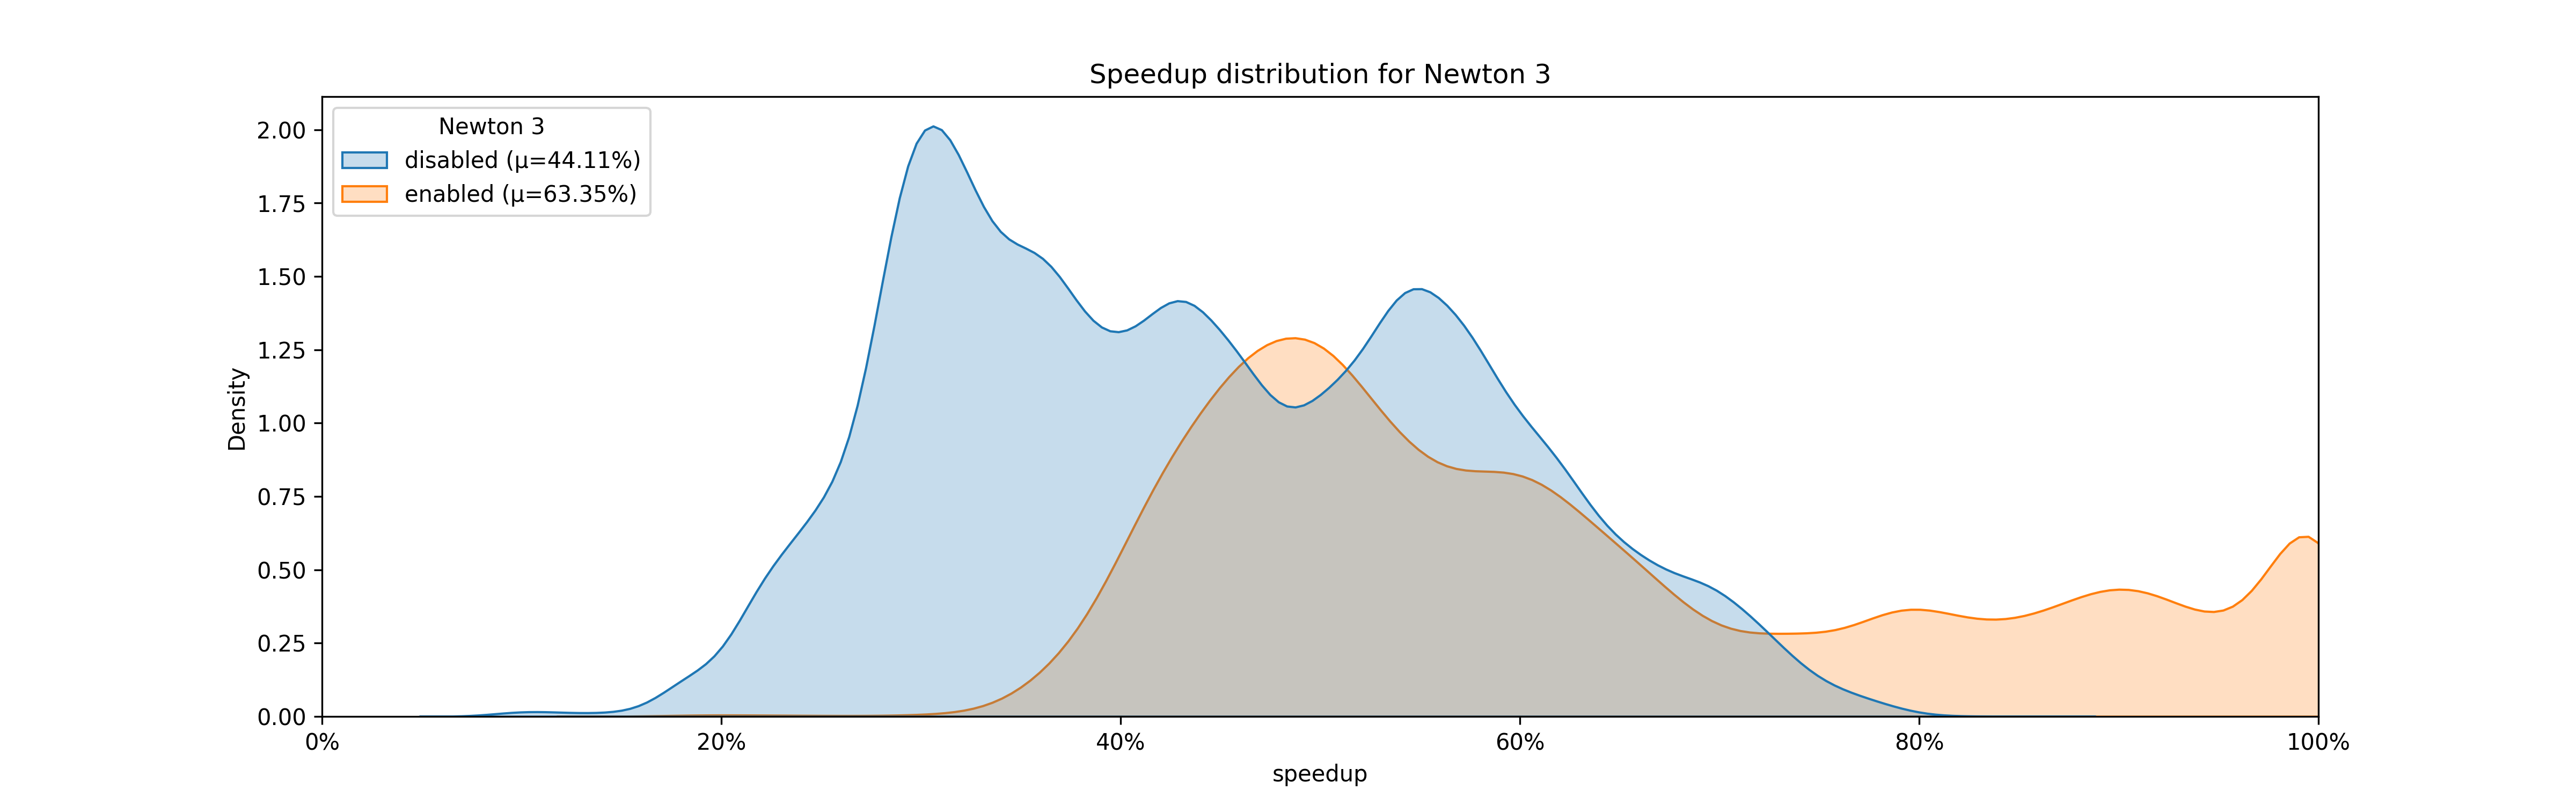
\includegraphics[width=\columnwidth,trim={1cm 0 2cm 1.5cm},clip]{figures/DataAnalytics/speedup_Newton 3.png}
    \caption[Speedup density plot based on the Newton 3 option]{Distribution of the relative speed based on the Newton 3 option. We can see that enabling Newton3 is generally the better option, allowing for higher relative speeds. Therefore, we can confirm that Newton 3 is generally a good option to enable.}
    \label{fig:inputAnalysisDensityNewton3}
  \end{subfigure}

  \vspace{0.2cm}

  \begin{subfigure}{\columnwidth}
    \centering
    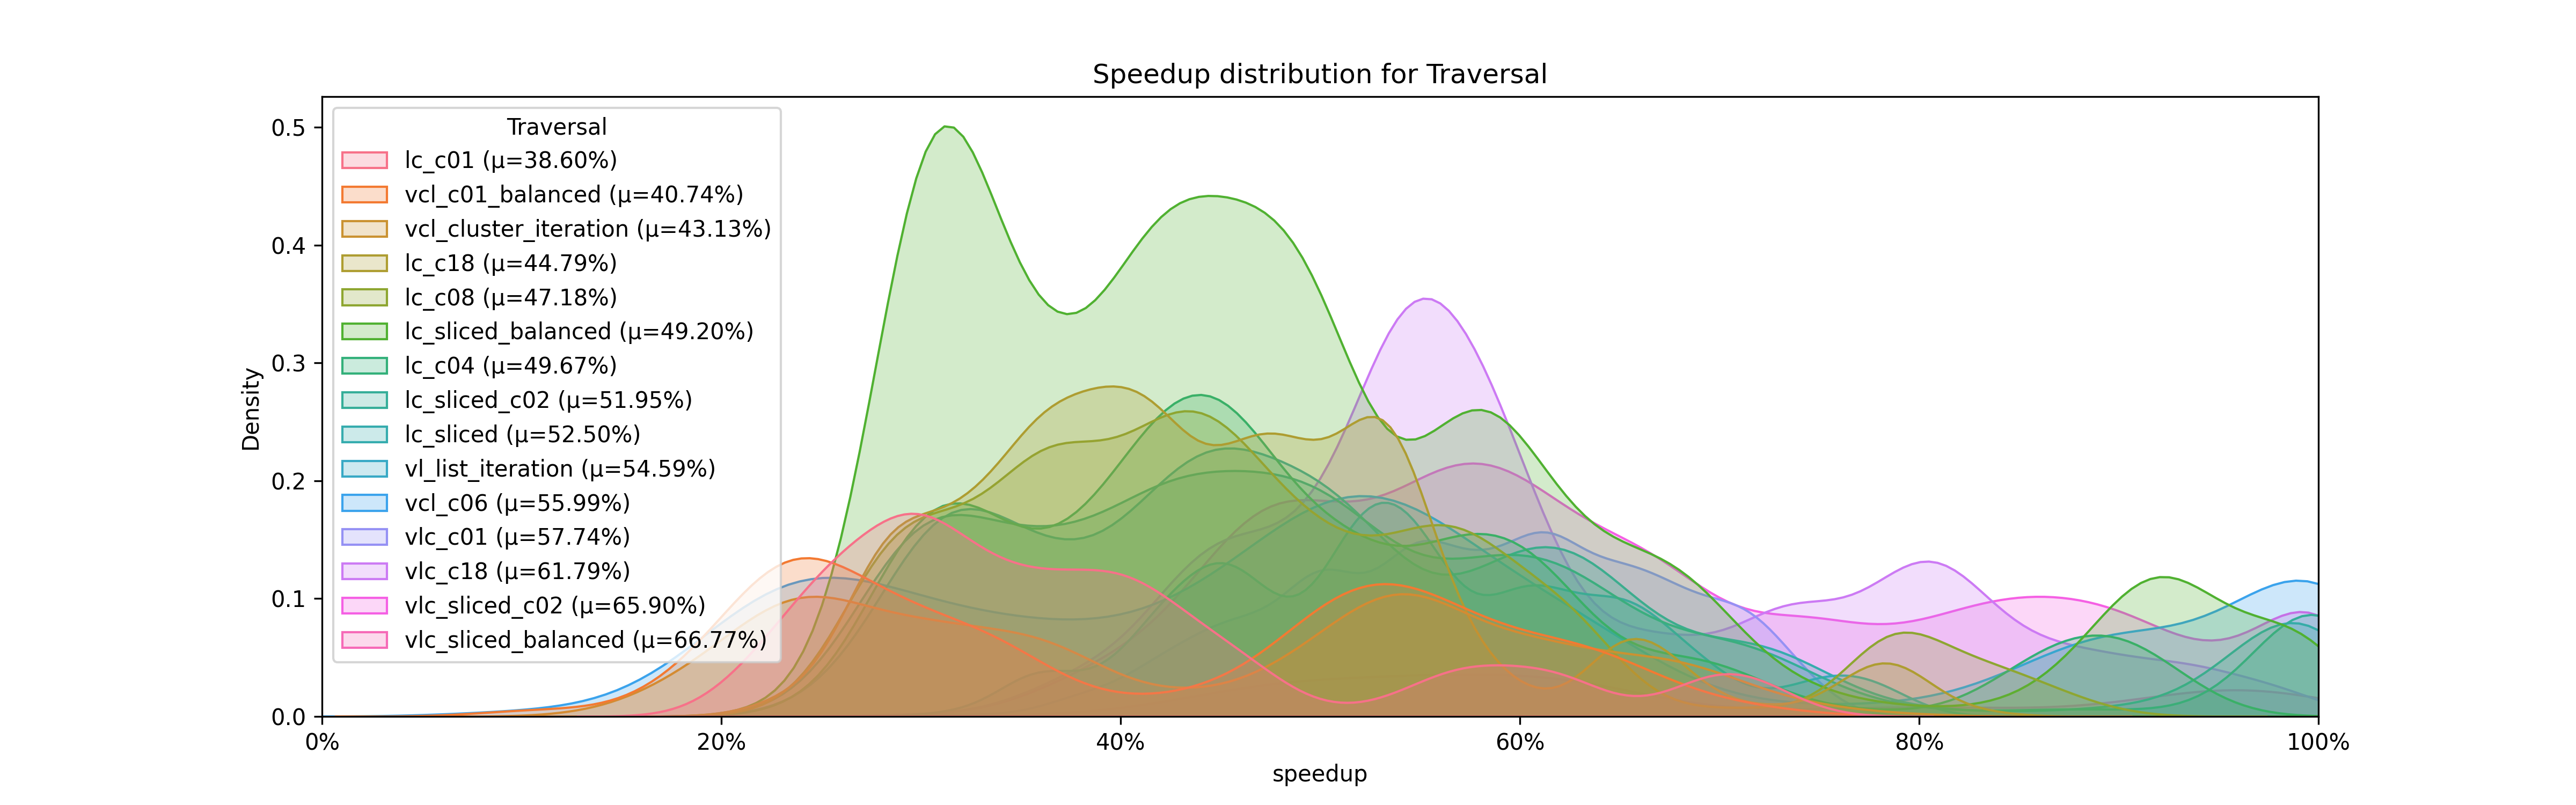
\includegraphics[width=\columnwidth,trim={1cm 0 2cm 1.5cm},clip]{figures/DataAnalytics/speedup_Traversal.png}
    \caption[Speedup density plot based on the Traversal option]{Distribution of the relative speed based on the Traversal option.  The vlc\_sliced\_balanced option generally performed better than the other options with an expected relative speed of 66\%.}
    \label{fig:inputAnalysisDensityTraversal}
  \end{subfigure}

  \vspace{0.2cm}

  \begin{subfigure}{\columnwidth}
    \centering
    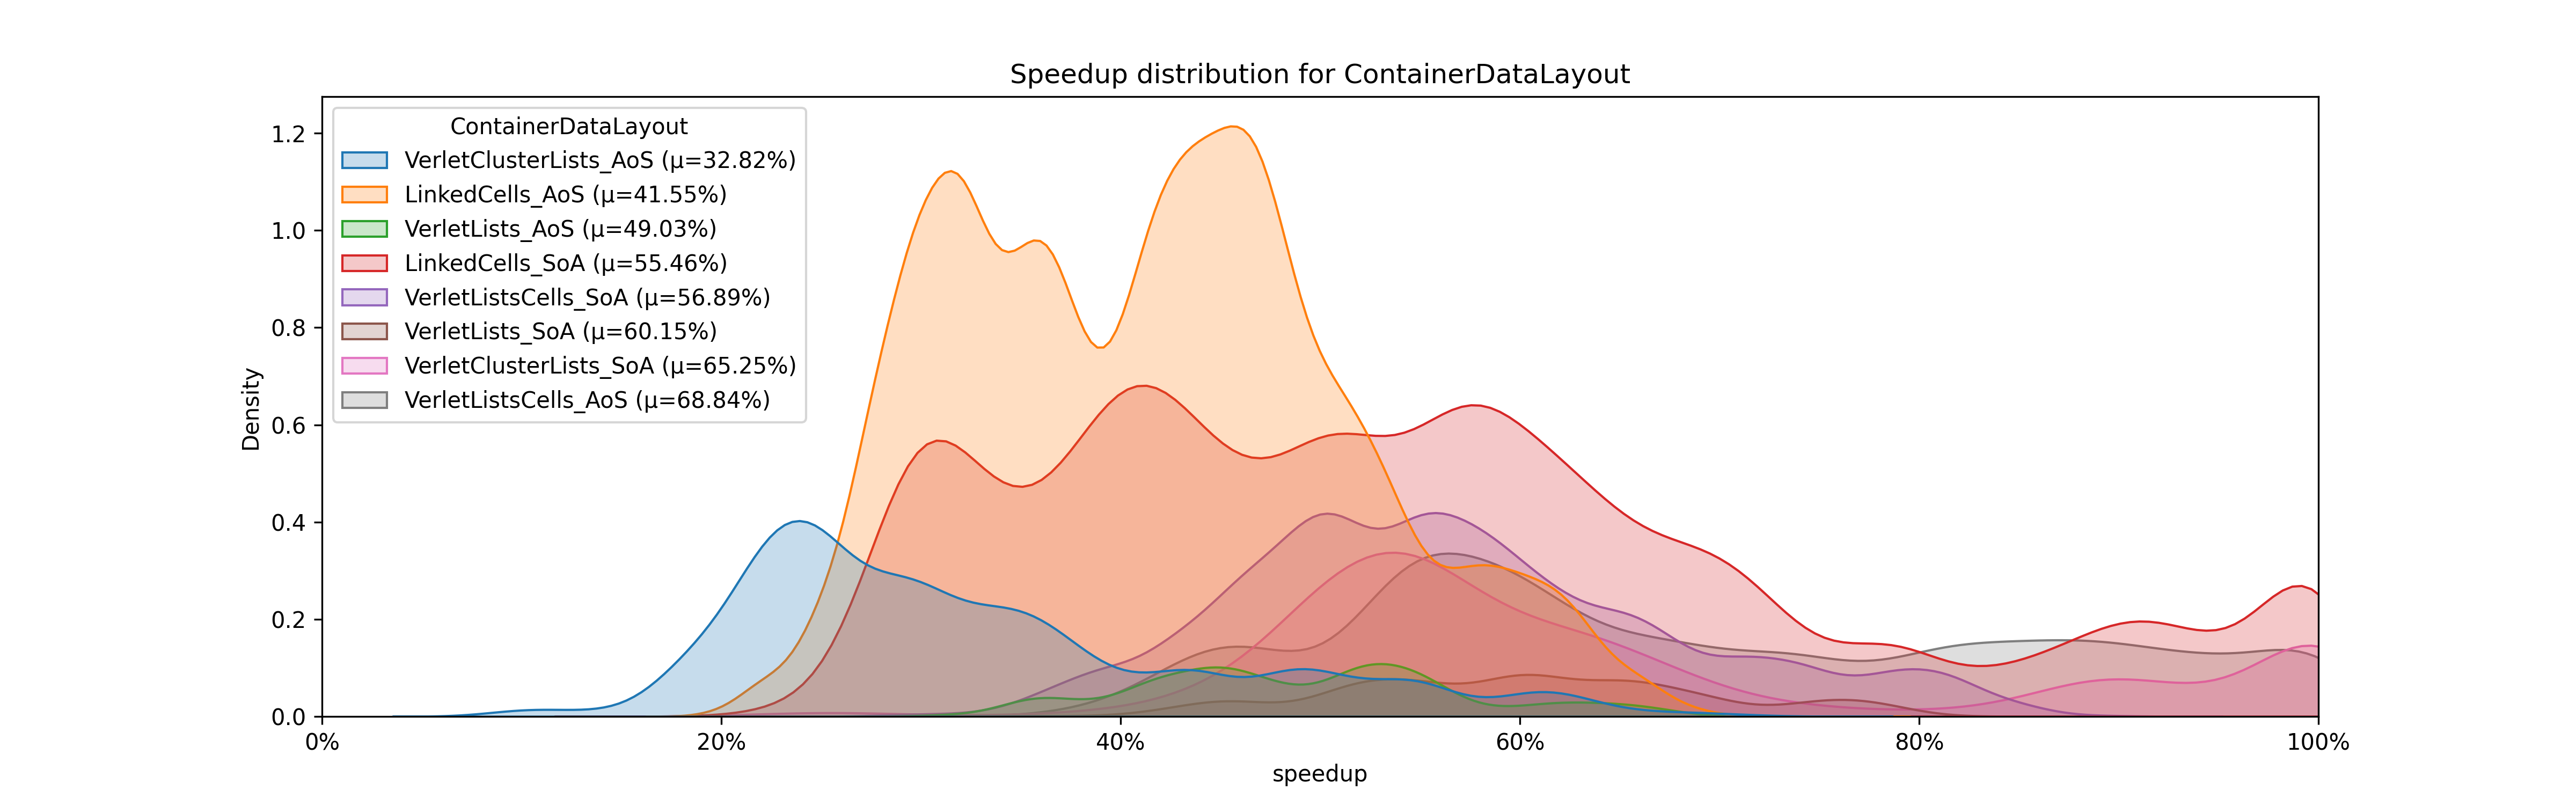
\includegraphics[width=\columnwidth,trim={1cm 0 2cm 1.5cm},clip]{figures/DataAnalytics/speedup_ContainerDataLayout.png}
    \caption[Speedup density plot of Configuration-Datalayout option]{Distribution of the relative speed based on the ContainerDatalayout option. The VerletListCells\_AoS ContainerDatalayout performed best with an expected relative speed of 68.8\%.}
    \label{fig:inputAnalysisDensityDatalayout}
  \end{subfigure}

  \caption[Speedup density plots based on different configuration options]{Density plots showing the relative speed distribution based on different configuration options for the collected dataset.}
  \label{fig:inputAnalysisDensity}
\end{figure}
